% Chapter 3 -- Statistics for Noisy Returns
% Requires: amsmath, amssymb, booktabs, array, tabularx, graphicx, tcolorbox (breakable, skins), hyperref or url.
% Defines the callout box only if the preamble has not.
\providecolor{fenavy}{HTML}{1B2A6B}
\providecolor{feshade}{HTML}{F3F5FA}
\makeatletter
\@ifundefined{callout}{%
  \newtcolorbox{callout}{breakable, enhanced,
    colback=white, colframe=gray!70, boxrule=0.5pt, arc=1mm,
    borderline west={2.5pt}{0pt}{gray!70},
    left=8pt, right=8pt, top=4pt, bottom=4pt}%
}{}
\makeatother

\chapter{Statistics for Noisy Returns}
\label{ch:03}

Part II of the book turns the lessons of Part I into tools. It begins with the most basic tool of all: the t-statistic\index{t-statistic}.

Almost every claim in quantitative finance ends in a test statistic\index{hypothesis testing!test statistic}, such as ``the strategy's alpha\index{alpha} has a t-statistic of 2.4.'' A t-statistic is an estimate, such as a mean return or an alpha, divided by its standard error\index{standard error}. It tells us how many standard errors the estimate lies away from zero, and a value above about 1.96 is usually read as significant at the 5\% level. 
That reading is only as good as the standard error behind it. The usual formula for the standard error, taught in introductory statistics (see, for example, Kuo 2025), assumes that \textbf{observations are independent}, that their \textbf{spread is constant over time}, and that their \textbf{distribution is roughly normal}.


Financial returns satisfy none of these assumptions exactly. Their tails are fat, their volatility\index{volatility} comes in clusters, and some of the most popular research designs build strong dependence between observations. When these assumptions fail, the standard error is often too small, so the t-statistic looks larger than it should, and a result can appear significant when it is not. The good news is that each of these problems has a well-tested remedy, and this chapter shows you how to choose the right one.

The claim on trial\index{claims-on-trial method} in this chapter is one that every researcher relies on: \textbf{with the right standard errors, regression statistics are reliable for financial returns.} Is that true, and if so, which standard errors are the right ones?

By the end of the chapter you will be able to:

\begin{itemize}
  \item summarize a return distribution by its mean, variance\index{variance}, skewness\index{skewness}, kurtosis\index{kurtosis} and autocorrelation\index{autocorrelation};
  \item run and interpret a linear regression, including its slope, intercept and $R^2$\index{regression!R-squared@$R^2$}, and explain what heteroskedasticity\index{heteroskedasticity} and serial correlation do to its standard errors;
  \item explain the CAPM\index{capital asset pricing model (CAPM)} and the Fama--French\index{Fama--French factors} three-factor model, and interpret beta\index{beta} and alpha;
  \item describe the stylized facts\index{stylized facts of returns} of financial returns: fat tails\index{fat tails}, volatility clustering\index{volatility clustering}, weak autocorrelation and asymmetry;
  \item choose standard errors that remain valid when those features\index{features and targets} are present: White, Newey--West\index{standard error!Newey--West (HAC)} and clustered errors;
  \item explain why overlapping long-horizon regressions mislead, and how to correct them;
  \item use the bootstrap\index{bootstrap} to measure uncertainty without relying on normality;
  \item test whether the best of many strategies truly beats a benchmark with White's reality check\index{White's reality check};
  \item separate statistical significance\index{statistical significance} from economic significance\index{economic significance}.
\end{itemize}

In the lab you will measure these features on nearly a century of real data, compute the alphas of 25 classic portfolios four different ways, and run a controlled experiment that shows how often overlapping regressions\index{overlapping observations} find predictability that is not there.

\section{Foundations: distributions, regression and factor models}
\label{sec:03-foundations}

\subsection{Describing a distribution}

Four numbers, called \textbf{moments}, summarize a return distribution.

\begin{itemize}
  \item The \textbf{mean} is its center: the average return.
  \item The \textbf{variance}\index{variance|textbf}, or its square root the standard deviation\index{standard deviation}, measures spread: how far returns typically fall from the mean.
  \item \textbf{Skewness}\index{skewness|textbf} measures asymmetry. It is negative when large losses are more likely than large gains of the same size, as for most stock indexes.
  \item \textbf{Kurtosis}\index{kurtosis|textbf} measures how heavy the tails are. A normal distribution\index{distribution!normal} has kurtosis 3; values above 3 indicate \textbf{fat tails}\index{fat tails|textbf}, meaning extreme returns occur more often than a normal distribution predicts.
\end{itemize}

Figure~\ref{fig:03-moments} shows what each of the four moments changes, by comparing the normal distribution with one that differs in that moment alone.

\begin{figure}[htbp]
\centering
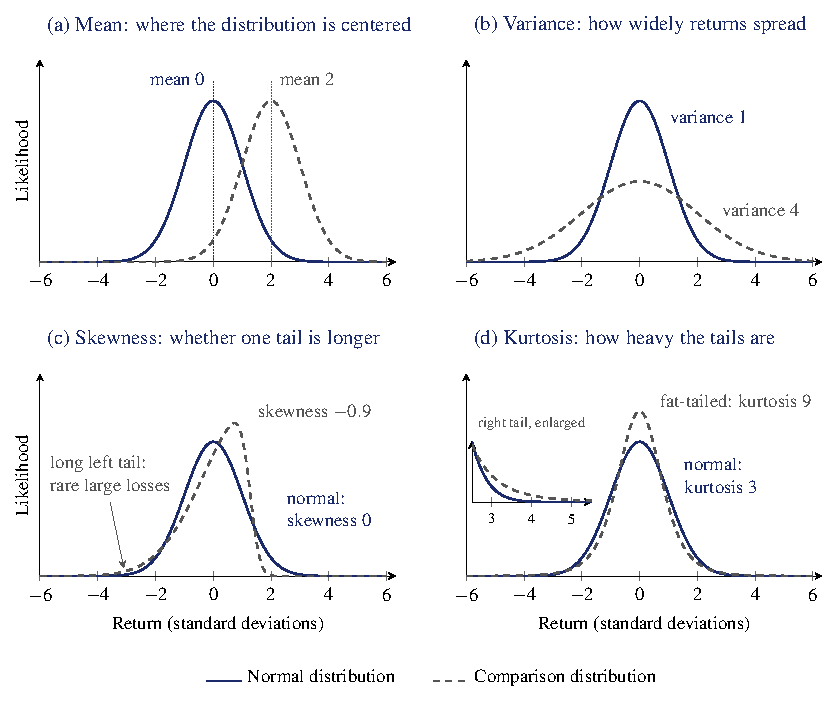
\includegraphics[width=0.7\linewidth]{images/fig03-0-moments.pdf}
\caption{The four moments of a distribution. Each panel compares the standard normal distribution (solid) with one that differs in a single respect. (a)~The mean sets the center. (b)~The variance sets the spread. (c)~Negative skewness lengthens the left tail, so large losses are more likely than large gains of the same size. (d)~Higher kurtosis puts more weight in the tails: the normal distribution has kurtosis 3, the fat-tailed one shown has kurtosis 9. Panels (c) and (d) keep the mean and variance of the normal distribution.}
\label{fig:03-moments}
\end{figure}

A fifth measure describes behavior over time. \textbf{Autocorrelation}\index{autocorrelation|textbf} is the correlation\index{correlation} of a series with its own past values: the first-order autocorrelation compares each month with the month before. A return series with zero autocorrelation cannot be predicted from its own history.

\subsection{Linear regression}
\label{sec:03-regression}

A regression describes how one variable, $y$, moves with another, $x$. Ordinary least squares\index{regression!ordinary least squares (OLS)} (OLS) fits
\begin{equation}
  y_t = \alpha + \beta x_t + \varepsilon_t
  \label{eq:03-ols}
\end{equation}
by choosing the intercept $\alpha$ and slope $\beta$ that make the \textbf{residuals}\index{regression!residuals|textbf} $\varepsilon_t$, the gaps between the actual values and the fitted line, as small as possible in the sense of their sum of squares. The slope $\beta$ measures how much $y$ moves when $x$ moves by one unit. The \textbf{R-squared}\index{regression!R-squared@$R^2$|textbf}, $R^2$, is the share of the variance of $y$ that the regression explains, from 0 (none) to 1 (all).

Each estimate comes with a standard error, and the usual formula for it assumes that the residuals are independent of one another and have the same variance throughout. Two departures from these assumptions are common in finance:

\begin{itemize}
  \item \textbf{Heteroskedasticity}\index{heteroskedasticity|textbf}: the variance of the residuals changes over time or across observations, for example rising in a crisis.
  \item \textbf{Serial correlation}: residuals are correlated with their own past values, so one large error tends to be followed by another.
\end{itemize}

When either is present, the coefficient estimates usually remain reasonable, but the usual standard errors are wrong, and the corrections developed in this chapter are needed.

Figure~\ref{fig:03-hetero-scatter} shows heteroskedasticity across observations, following Kuo (2025, Figure 15.4). The two panels\index{panel data} share the same true line, but on the right the scatter of the points grows as $x$ grows. Figure~\ref{fig:03-residual-problems} shows both problems in the form they usually take in finance, over time. In panel~(a) the residuals become much larger during a crisis, and in panel~(b) they drift above or below zero in long runs.

\begin{figure}[!htbp]
  \centering
  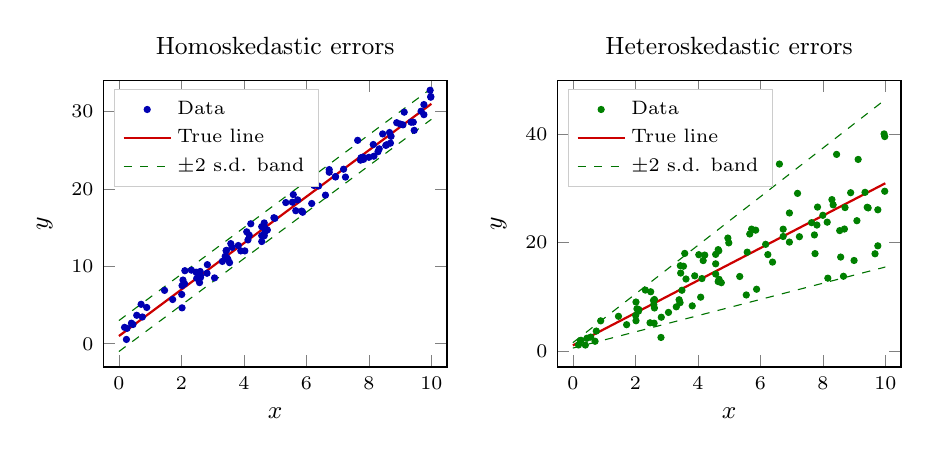
\begin{tikzpicture}
  \begin{axis}[
    name=ph,
    scale only axis, width=0.36\linewidth, height=0.3\linewidth,
    xmin=-0.5, xmax=10.5, ymin=-3, ymax=34,
    xtick={0,2,...,10},
    tick label style={font=\scriptsize}, label style={font=\small},
    xlabel={$x$}, ylabel={$y$},
    title={Homoskedastic errors}, title style={font=\small},
    legend style={font=\scriptsize, at={(0.03,0.97)}, anchor=north west, draw=gray!40},
    legend cell align=left,
  ]
    \addplot[only marks, mark=*, mark size=1.1pt, blue!70!black] coordinates {(0.18,2.12) (0.24,0.56) (0.26,1.99) (0.40,2.66) (0.45,2.49) (0.57,3.68) (0.71,5.10) (0.75,3.46) (0.89,4.69) (1.46,6.90) (1.72,5.72) (2.01,6.37) (2.02,4.64) (2.02,7.51) (2.05,8.23) (2.10,7.75) (2.11,9.44) (2.32,9.51) (2.47,9.25) (2.49,8.45) (2.58,7.90) (2.59,8.90) (2.60,9.34) (2.61,8.79) (2.61,8.56) (2.82,9.11) (2.83,10.22) (3.06,8.51) (3.31,10.64) (3.40,11.29) (3.43,12.01) (3.44,12.07) (3.45,11.16) (3.49,10.91) (3.54,10.48) (3.58,12.94) (3.62,12.46) (3.82,12.69) (3.90,12.00) (4.03,12.00) (4.09,14.46) (4.13,13.42) (4.17,14.03) (4.22,15.50) (4.57,13.21) (4.57,13.97) (4.57,15.13) (4.65,15.61) (4.65,13.95) (4.67,14.97) (4.68,14.47) (4.75,14.70) (4.96,16.28) (4.99,16.20) (5.34,18.24) (5.55,18.29) (5.58,19.27) (5.66,17.19) (5.72,18.59) (5.85,17.14) (5.88,16.99) (6.17,18.12) (6.24,20.45) (6.39,20.38) (6.61,19.20) (6.73,22.50) (6.73,22.16) (6.93,21.60) (6.93,21.55) (7.19,22.55) (7.25,21.53) (7.64,26.28) (7.73,23.72) (7.75,24.04) (7.81,24.12) (7.83,23.83) (8.00,24.09) (8.14,25.74) (8.16,24.23) (8.29,24.81) (8.33,25.18) (8.44,27.11) (8.54,25.63) (8.57,25.71) (8.66,27.29) (8.69,25.92) (8.71,26.80) (8.89,28.56) (9.00,28.39) (9.09,28.28) (9.13,29.92) (9.35,28.62) (9.42,28.63) (9.45,27.57) (9.67,30.04) (9.76,30.90) (9.76,29.60) (9.96,32.75) (9.98,31.95) (9.98,31.85)};
    \addlegendentry{Data}
    \addplot[red!80!black, thick, domain=0:10, samples=2] {1+3*x};
    \addlegendentry{True line}
    \addplot[green!45!black, dashed, domain=0:10, samples=2] {1+3*x+2};
    \addlegendentry{$\pm 2$ s.d. band}
    \addplot[green!45!black, dashed, domain=0:10, samples=2, forget plot] {1+3*x-2};
  \end{axis}
  \begin{axis}[
    at={(ph.east)}, anchor=west, xshift=1.4cm,
    name=pt,
    scale only axis, width=0.36\linewidth, height=0.3\linewidth,
    xmin=-0.5, xmax=10.5, ymin=-3, ymax=50,
    xtick={0,2,...,10},
    tick label style={font=\scriptsize}, label style={font=\small},
    xlabel={$x$}, ylabel={$y$},
    title={Heteroskedastic errors}, title style={font=\small},
    legend style={font=\scriptsize, at={(0.03,0.97)}, anchor=north west, draw=gray!40},
    legend cell align=left,
  ]
    \addplot[only marks, mark=*, mark size=1.1pt, green!50!black] coordinates {(0.18,1.08) (0.24,1.85) (0.26,1.94) (0.40,1.06) (0.45,2.32) (0.57,2.53) (0.71,1.76) (0.75,3.65) (0.89,5.54) (1.46,6.38) (1.72,4.83) (2.01,6.54) (2.02,9.02) (2.02,5.56) (2.05,7.77) (2.10,7.33) (2.11,7.63) (2.32,11.23) (2.47,5.18) (2.49,10.92) (2.58,9.31) (2.59,8.54) (2.60,5.11) (2.61,9.49) (2.61,7.92) (2.82,2.47) (2.83,6.21) (3.06,7.10) (3.31,8.13) (3.40,9.44) (3.43,8.90) (3.44,15.74) (3.45,14.38) (3.49,11.20) (3.54,15.65) (3.58,18.02) (3.62,13.28) (3.82,8.31) (3.90,13.87) (4.03,17.78) (4.09,9.92) (4.13,13.36) (4.17,16.69) (4.22,17.71) (4.57,17.84) (4.57,16.09) (4.57,14.20) (4.65,12.81) (4.65,18.72) (4.67,18.50) (4.68,13.21) (4.75,12.60) (4.96,20.86) (4.99,19.97) (5.34,13.75) (5.55,10.33) (5.58,18.25) (5.66,21.61) (5.72,22.51) (5.85,22.32) (5.88,11.39) (6.17,19.70) (6.24,17.80) (6.39,16.41) (6.61,34.55) (6.73,21.15) (6.73,22.50) (6.93,20.11) (6.93,25.50) (7.19,29.13) (7.25,21.11) (7.64,23.71) (7.73,21.44) (7.75,17.98) (7.81,23.27) (7.83,26.59) (8.00,25.07) (8.14,23.80) (8.16,13.44) (8.29,27.97) (8.33,27.00) (8.44,36.34) (8.54,22.24) (8.57,17.34) (8.66,13.79) (8.69,22.53) (8.71,26.50) (8.89,29.25) (9.00,16.71) (9.09,24.07) (9.13,35.41) (9.35,29.32) (9.42,26.56) (9.45,26.44) (9.67,17.95) (9.76,19.42) (9.76,26.09) (9.96,40.13) (9.98,39.64) (9.98,29.52)};
    \addlegendentry{Data}
    \addplot[red!80!black, thick, domain=0:10, samples=2] {1+3*x};
    \addlegendentry{True line}
    \addplot[green!45!black, dashed, domain=0:10, samples=2] {(1+3*x)*1.5};
    \addlegendentry{$\pm 2$ s.d. band}
    \addplot[green!45!black, dashed, domain=0:10, samples=2, forget plot] {(1+3*x)*0.5};
  \end{axis}
  \end{tikzpicture}
  \caption{Homoskedastic and heteroskedastic errors around the same true line, $y = 1 + 3x$, shown with simulated data. On the left, the scatter around the line has the same width everywhere, so the dashed bands run parallel to the line. On the right, the scatter grows with $x$, so the bands fan out. The fitted line is unbiased in both cases, but on the right the usual standard error understates the uncertainty. After Kuo (2025, Figure 15.4).}
  \label{fig:03-hetero-scatter}
\end{figure}

\begin{figure}[!htbp]
  \centering
  \begin{tikzpicture}
  % Panel (a): heteroskedasticity
  \begin{axis}[
    name=pa,
    scale only axis, width=0.55\linewidth, height=0.17\linewidth,
    axis lines=left, axis line style={-stealth, thin},
    xmin=0, xmax=205, ymin=-7.5, ymax=7.5,
    xtick=\empty, ytick={-5,0,5},
    tick label style={font=\small}, label style={font=\small},
    ylabel={Residual},
    title={(a) Heteroskedasticity: the spread changes},
    title style={font=\small, anchor=south west, at={(0,1)}, xshift=-4pt},
    clip=false,
  ]
    % Plus or minus two standard deviations
    \addplot[name path=up, gray!60, thin] coordinates {(1,2.00) (2,2.00) (3,2.00) (4,2.00) (5,2.00) (6,2.00) (7,2.00) (8,2.00) (9,2.00) (10,2.00) (11,2.00) (12,2.00) (13,2.00) (14,2.00) (15,2.00) (16,2.00) (17,2.00) (18,2.00) (19,2.00) (20,2.00) (21,2.00) (22,2.00) (23,2.00) (24,2.00) (25,2.00) (26,2.00) (27,2.00) (28,2.00) (29,2.00) (30,2.00) (31,2.00) (32,2.00) (33,2.00) (34,2.00) (35,2.00) (36,2.00) (37,2.00) (38,2.00) (39,2.00) (40,2.00) (41,2.00) (42,2.00) (43,2.00) (44,2.00) (45,2.00) (46,2.00) (47,2.00) (48,2.00) (49,2.00) (50,2.00) (51,2.00) (52,2.00) (53,2.00) (54,2.00) (55,2.00) (56,2.00) (57,2.00) (58,2.00) (59,2.00) (60,2.00) (61,2.00) (62,2.00) (63,2.00) (64,2.00) (65,2.00) (66,2.00) (67,2.00) (68,2.00) (69,2.00) (70,2.00) (71,2.00) (72,2.00) (73,2.00) (74,2.00) (75,2.00) (76,2.00) (77,2.00) (78,2.00) (79,2.00) (80,2.00) (81,2.00) (82,2.00) (83,2.00) (84,2.00) (85,2.00) (86,2.00) (87,2.00) (88,2.00) (89,2.00) (90,2.00) (91,2.00) (92,2.00) (93,2.00) (94,2.00) (95,2.00) (96,2.00) (97,2.00) (98,2.00) (99,2.00) (100,2.00) (101,2.00) (102,2.00) (103,2.00) (104,2.00) (105,2.00) (106,2.00) (107,2.57) (108,3.14) (109,3.71) (110,4.29) (111,4.86) (112,5.43) (113,6.00) (114,6.00) (115,6.00) (116,6.00) (117,6.00) (118,6.00) (119,6.00) (120,6.00) (121,6.00) (122,6.00) (123,6.00) (124,6.00) (125,6.00) (126,6.00) (127,6.00) (128,6.00) (129,6.00) (130,6.00) (131,6.00) (132,6.00) (133,6.00) (134,6.00) (135,6.00) (136,6.00) (137,6.00) (138,5.43) (139,4.86) (140,4.29) (141,3.71) (142,3.14) (143,2.57) (144,2.00) (145,2.00) (146,2.00) (147,2.00) (148,2.00) (149,2.00) (150,2.00) (151,2.00) (152,2.00) (153,2.00) (154,2.00) (155,2.00) (156,2.00) (157,2.00) (158,2.00) (159,2.00) (160,2.00) (161,2.00) (162,2.00) (163,2.00) (164,2.00) (165,2.00) (166,2.00) (167,2.00) (168,2.00) (169,2.00) (170,2.00) (171,2.00) (172,2.00) (173,2.00) (174,2.00) (175,2.00) (176,2.00) (177,2.00) (178,2.00) (179,2.00) (180,2.00) (181,2.00) (182,2.00) (183,2.00) (184,2.00) (185,2.00) (186,2.00) (187,2.00) (188,2.00) (189,2.00) (190,2.00) (191,2.00) (192,2.00) (193,2.00) (194,2.00) (195,2.00) (196,2.00) (197,2.00) (198,2.00) (199,2.00) (200,2.00)};
    \addplot[name path=lo, gray!60, thin] coordinates {(1,-2.00) (2,-2.00) (3,-2.00) (4,-2.00) (5,-2.00) (6,-2.00) (7,-2.00) (8,-2.00) (9,-2.00) (10,-2.00) (11,-2.00) (12,-2.00) (13,-2.00) (14,-2.00) (15,-2.00) (16,-2.00) (17,-2.00) (18,-2.00) (19,-2.00) (20,-2.00) (21,-2.00) (22,-2.00) (23,-2.00) (24,-2.00) (25,-2.00) (26,-2.00) (27,-2.00) (28,-2.00) (29,-2.00) (30,-2.00) (31,-2.00) (32,-2.00) (33,-2.00) (34,-2.00) (35,-2.00) (36,-2.00) (37,-2.00) (38,-2.00) (39,-2.00) (40,-2.00) (41,-2.00) (42,-2.00) (43,-2.00) (44,-2.00) (45,-2.00) (46,-2.00) (47,-2.00) (48,-2.00) (49,-2.00) (50,-2.00) (51,-2.00) (52,-2.00) (53,-2.00) (54,-2.00) (55,-2.00) (56,-2.00) (57,-2.00) (58,-2.00) (59,-2.00) (60,-2.00) (61,-2.00) (62,-2.00) (63,-2.00) (64,-2.00) (65,-2.00) (66,-2.00) (67,-2.00) (68,-2.00) (69,-2.00) (70,-2.00) (71,-2.00) (72,-2.00) (73,-2.00) (74,-2.00) (75,-2.00) (76,-2.00) (77,-2.00) (78,-2.00) (79,-2.00) (80,-2.00) (81,-2.00) (82,-2.00) (83,-2.00) (84,-2.00) (85,-2.00) (86,-2.00) (87,-2.00) (88,-2.00) (89,-2.00) (90,-2.00) (91,-2.00) (92,-2.00) (93,-2.00) (94,-2.00) (95,-2.00) (96,-2.00) (97,-2.00) (98,-2.00) (99,-2.00) (100,-2.00) (101,-2.00) (102,-2.00) (103,-2.00) (104,-2.00) (105,-2.00) (106,-2.00) (107,-2.57) (108,-3.14) (109,-3.71) (110,-4.29) (111,-4.86) (112,-5.43) (113,-6.00) (114,-6.00) (115,-6.00) (116,-6.00) (117,-6.00) (118,-6.00) (119,-6.00) (120,-6.00) (121,-6.00) (122,-6.00) (123,-6.00) (124,-6.00) (125,-6.00) (126,-6.00) (127,-6.00) (128,-6.00) (129,-6.00) (130,-6.00) (131,-6.00) (132,-6.00) (133,-6.00) (134,-6.00) (135,-6.00) (136,-6.00) (137,-6.00) (138,-5.43) (139,-4.86) (140,-4.29) (141,-3.71) (142,-3.14) (143,-2.57) (144,-2.00) (145,-2.00) (146,-2.00) (147,-2.00) (148,-2.00) (149,-2.00) (150,-2.00) (151,-2.00) (152,-2.00) (153,-2.00) (154,-2.00) (155,-2.00) (156,-2.00) (157,-2.00) (158,-2.00) (159,-2.00) (160,-2.00) (161,-2.00) (162,-2.00) (163,-2.00) (164,-2.00) (165,-2.00) (166,-2.00) (167,-2.00) (168,-2.00) (169,-2.00) (170,-2.00) (171,-2.00) (172,-2.00) (173,-2.00) (174,-2.00) (175,-2.00) (176,-2.00) (177,-2.00) (178,-2.00) (179,-2.00) (180,-2.00) (181,-2.00) (182,-2.00) (183,-2.00) (184,-2.00) (185,-2.00) (186,-2.00) (187,-2.00) (188,-2.00) (189,-2.00) (190,-2.00) (191,-2.00) (192,-2.00) (193,-2.00) (194,-2.00) (195,-2.00) (196,-2.00) (197,-2.00) (198,-2.00) (199,-2.00) (200,-2.00)};
    \addplot[fenavy!12] fill between[of=up and lo];
    \draw[gray!70, thin] (axis cs:0,0) -- (axis cs:200,0);
    \addplot[fenavy, thin, mark=none] coordinates {(1,0.00) (2,0.30) (3,-0.27) (4,-0.89) (5,-0.45) (6,-0.99) (7,0.06) (8,1.34) (9,-0.49) (10,-0.62) (11,0.49) (12,0.36) (13,0.11) (14,-0.93) (15,-0.03) (16,0.70) (17,-1.34) (18,-0.46) (19,-1.90) (20,-1.29) (21,-1.84) (22,-0.24) (23,-1.27) (24,0.27) (25,0.16) (26,-0.19) (27,-2.52) (28,-0.54) (29,-0.05) (30,0.11) (31,-1.53) (32,-0.48) (33,-0.98) (34,-0.81) (35,1.06) (36,-0.81) (37,-0.03) (38,0.88) (39,-0.58) (40,-0.11) (41,0.11) (42,0.06) (43,-1.23) (44,0.08) (45,1.36) (46,-1.55) (47,0.86) (48,0.12) (49,-0.64) (50,2.00) (51,0.76) (52,-1.20) (53,0.07) (54,0.58) (55,-0.19) (56,0.68) (57,-0.07) (58,0.67) (59,1.44) (60,-0.68) (61,0.20) (62,-0.46) (63,0.13) (64,-1.19) (65,-0.58) (66,-0.20) (67,0.90) (68,1.15) (69,-1.32) (70,-0.79) (71,0.65) (72,-1.99) (73,-0.46) (74,-0.10) (75,1.26) (76,0.69) (77,-0.33) (78,-0.37) (79,-0.25) (80,1.52) (81,-0.43) (82,-0.30) (83,0.35) (84,-0.12) (85,-0.20) (86,-1.11) (87,-0.01) (88,-0.44) (89,1.17) (90,0.65) (91,-0.02) (92,0.67) (93,-0.34) (94,1.05) (95,-0.01) (96,0.58) (97,-1.29) (98,0.35) (99,-1.69) (100,-2.04) (101,-0.30) (102,-0.90) (103,0.16) (104,2.24) (105,-0.83) (106,-0.62) (107,0.26) (108,0.77) (109,-0.33) (110,-0.44) (111,1.71) (112,1.41) (113,-3.10) (114,-0.24) (115,0.11) (116,-3.16) (117,0.78) (118,-2.57) (119,2.92) (120,0.58) (121,0.27) (122,-1.77) (123,-0.36) (124,-5.99) (125,-3.39) (126,1.09) (127,-6.39) (128,2.54) (129,-5.24) (130,2.27) (131,-2.54) (132,2.34) (133,0.39) (134,-4.61) (135,3.75) (136,4.33) (137,-0.20) (138,-0.74) (139,-0.39) (140,-2.09) (141,2.04) (142,-0.85) (143,-0.07) (144,-0.79) (145,-0.63) (146,-1.28) (147,1.26) (148,-0.15) (149,0.97) (150,0.01) (151,-0.69) (152,-0.33) (153,-0.56) (154,0.01) (155,-0.38) (156,-0.30) (157,-1.38) (158,-0.81) (159,1.65) (160,-0.67) (161,-1.05) (162,0.34) (163,1.41) (164,-1.45) (165,-0.21) (166,-0.63) (167,-1.76) (168,0.73) (169,-0.02) (170,0.07) (171,-0.75) (172,0.45) (173,-0.54) (174,-0.14) (175,-1.11) (176,-1.22) (177,1.34) (178,-0.51) (179,0.29) (180,-0.03) (181,-0.44) (182,-0.51) (183,0.63) (184,-0.30) (185,-0.15) (186,0.02) (187,1.18) (188,0.68) (189,0.38) (190,-0.56) (191,-1.38) (192,0.95) (193,0.97) (194,-0.14) (195,0.54) (196,0.78) (197,0.83) (198,0.92) (199,-0.46) (200,1.51)};
    \node[font=\footnotesize, anchor=south] at (axis cs:125,6.2) {crisis: large errors};
    \node[font=\footnotesize, anchor=south, gray!60!black] at (axis cs:50,2.6) {calm: small errors};
  \end{axis}

  % Panel (b): serial correlation
  \begin{axis}[
    at={(pa.south west)}, anchor=north west, yshift=-1.1cm,
    scale only axis, width=0.55\linewidth, height=0.17\linewidth,
    axis lines=left, axis line style={-stealth, thin},
    xmin=0, xmax=205, ymin=-4.5, ymax=4.5,
    xtick=\empty, ytick={-3,0,3},
    tick label style={font=\small}, label style={font=\small},
    xlabel={Time}, ylabel={Residual},
    title={(b) Serial correlation: errors come in runs},
    title style={font=\small, anchor=south west, at={(0,1)}, xshift=-4pt},
    clip=false,
  ]
    \draw[gray!70, thin] (axis cs:0,0) -- (axis cs:200,0);
    \addplot[fenavy, thin, mark=none] coordinates {(1,0.18) (2,0.60) (3,0.77) (4,1.12) (5,1.94) (6,2.43) (7,1.46) (8,0.35) (9,0.73) (10,0.09) (11,0.07) (12,0.50) (13,-0.44) (14,-1.49) (15,-1.13) (16,-0.93) (17,-0.92) (18,-0.77) (19,-1.10) (20,-1.74) (21,-1.56) (22,-1.84) (23,-2.43) (24,-1.80) (25,-1.56) (26,-1.11) (27,-1.47) (28,-1.59) (29,-1.88) (30,-2.07) (31,-1.65) (32,-1.82) (33,-1.36) (34,-0.97) (35,0.24) (36,-0.53) (37,0.02) (38,-0.03) (39,-0.04) (40,-0.79) (41,-0.92) (42,-0.39) (43,-0.37) (44,-0.27) (45,-0.39) (46,0.28) (47,0.23) (48,-0.97) (49,-1.19) (50,-2.05) (51,-3.45) (52,-3.21) (53,-2.03) (54,-1.70) (55,-2.06) (56,-2.25) (57,-1.32) (58,-1.04) (59,-0.85) (60,-0.75) (61,-0.62) (62,-0.10) (63,0.20) (64,0.29) (65,-0.31) (66,0.01) (67,-0.35) (68,0.28) (69,-0.43) (70,-0.44) (71,-0.38) (72,-1.02) (73,0.04) (74,0.80) (75,0.44) (76,0.78) (77,0.86) (78,-0.64) (79,-0.42) (80,-0.39) (81,-0.28) (82,-0.81) (83,-0.83) (84,-0.80) (85,-0.05) (86,0.13) (87,0.11) (88,0.90) (89,0.47) (90,0.19) (91,-0.79) (92,0.15) (93,0.64) (94,1.03) (95,1.22) (96,1.10) (97,1.05) (98,0.76) (99,0.54) (100,0.48) (101,1.21) (102,1.32) (103,1.09) (104,0.62) (105,0.19) (106,1.01) (107,1.13) (108,0.99) (109,0.66) (110,-0.02) (111,-0.05) (112,0.41) (113,0.15) (114,0.00) (115,-0.11) (116,-0.04) (117,-0.87) (118,-0.87) (119,-1.19) (120,-0.54) (121,-0.87) (122,-0.43) (123,0.44) (124,0.20) (125,-0.14) (126,-0.02) (127,-0.02) (128,-0.54) (129,-0.22) (130,0.88) (131,0.61) (132,0.41) (133,-0.20) (134,-0.00) (135,-0.66) (136,-1.14) (137,-0.30) (138,-0.73) (139,-0.05) (140,0.76) (141,0.78) (142,0.96) (143,1.84) (144,1.46) (145,0.93) (146,0.08) (147,0.09) (148,0.85) (149,1.23) (150,0.55) (151,0.02) (152,-0.25) (153,-0.06) (154,-0.16) (155,-0.02) (156,0.14) (157,-0.04) (158,-0.06) (159,0.06) (160,0.01) (161,0.27) (162,1.22) (163,1.35) (164,1.17) (165,0.11) (166,0.30) (167,-0.77) (168,-1.40) (169,-0.74) (170,-0.26) (171,-0.30) (172,-1.15) (173,-1.18) (174,-1.36) (175,-0.82) (176,0.49) (177,0.53) (178,0.04) (179,-0.58) (180,-0.52) (181,-0.54) (182,-1.06) (183,-0.84) (184,-1.32) (185,-0.54) (186,0.10) (187,0.66) (188,0.31) (189,0.53) (190,0.38) (191,0.12) (192,-0.07) (193,-0.75) (194,-1.40) (195,-0.77) (196,-0.75) (197,-0.53) (198,0.08) (199,-0.85) (200,-1.13)};
  \end{axis}
  \end{tikzpicture}
  \caption{Two ways regression residuals break the textbook assumptions, shown with simulated data. In panel~(a) the errors are independent, but their spread, shown by the shaded band of plus or minus two standard deviations, triples during a crisis. In panel~(b) the spread is constant, but each error is strongly correlated with the one before it, so positive and negative errors arrive in long runs. In both cases the usual standard error is wrong.}
  \label{fig:03-residual-problems}
\end{figure}


\subsection{The capital asset pricing model}
\label{sec:03-capm}

The capital asset pricing model (CAPM), developed independently by Sharpe (1964), Lintner (1965) and Mossin (1966), is one of the most important ideas in finance. Its central insight concerns which kind of risk investors are paid to bear. Before the CAPM, risk usually meant how much a single stock's price moved up and down. The CAPM showed that much of this movement can be removed by holding many stocks, which is called \textbf{diversification}\index{diversification|textbf}, so investors should not expect to be rewarded for bearing it. Only the part of risk that moves with the whole market cannot be diversified away, and only that part should earn a higher expected return\index{return!expected}. This split between \textbf{systematic risk}\index{risk!systematic|textbf}, which is rewarded, and \textbf{idiosyncratic risk}\index{risk!idiosyncratic|textbf}, which is not, still underlies almost all of asset pricing. The CAPM was also the first model to give a precise and testable answer to the central question of the field, which is why some assets earn more than others. Its implications reach far into practice. Companies use it to set the discount rate\index{discount rate} for investment projects, and surveys find that most finance officers rely on it to estimate their cost of capital (Graham and Harvey 2001). The idea of alpha, the return beyond what market exposure explains, comes directly from the model, and every alpha test in this book starts from it. Its conclusion that the market portfolio is the best risky portfolio for every investor also gave index funds their theoretical foundation.

Formally, the CAPM says that an asset's expected excess return\index{return!excess} is proportional to its \textbf{beta}\index{beta|textbf}, its sensitivity to the market:
\begin{equation}
  E[R_i] - r_f = \beta_i \left(E[R_m] - r_f\right), \qquad \beta_i = \frac{\operatorname{Cov}(R_i, R_m)}{\operatorname{Var}(R_m)}
  \label{eq:03-capm}
\end{equation}
Here $\operatorname{Cov}$ is the covariance, which measures how two returns move together, and $\operatorname{Var}$ is the variance. A stock with a beta of 1.5 tends to rise 1.5\% when the market rises 1\%, so it carries one and a half times the market's systematic risk and should earn one and a half times the market's excess return. The model is tested with a time-series regression of an asset's excess return on the market's excess return, as in Section~\ref{sec:01-foundations}. The slope of this regression estimates beta, and the intercept, \textbf{alpha}\index{alpha|textbf}, is the average return that the CAPM fails to explain. The model predicts that alpha is zero for every asset. Figure~\ref{fig:03-alpha} shows the two numbers on a scatter plot.

\providecolor{fenavy}{HTML}{1B2A6B}
\providecolor{fegray}{HTML}{4D4D4D}

\begin{figure}[!htbp]
  \centering
  \begin{tikzpicture}[
    % Fitted regression: strategy = 1.16 + 1.15 * market
    declare function={fit(\x) = 1.16 + 1.15*\x;  zero(\x) = 1.15*\x;}
  ]
  \begin{axis}[
    scale only axis, width=0.41\linewidth, height=0.29\linewidth,
    axis lines=left,
    axis line style={-stealth, thin},
    xmin=-11, xmax=12.5, ymin=-12.5, ymax=16,
    xtick={-8,-4,0,4,8,12},
    ytick={-10,-5,0,5,10,15},
    tick label style={font=\footnotesize}, label style={font=\small},
    xlabel={Market excess return, $R_m - r_f$ (\% a month)},
    ylabel={Strategy excess return (\%)},
    clip=false,
  ]
    % Reference axes through zero
    \draw[gray!40] (axis cs:-11,0) -- (axis cs:12.5,0);
    \draw[gray!40] (axis cs:0,-12.5) -- (axis cs:0,16);

    % Monthly observations (illustrative)
    \addplot[only marks, mark=*, mark size=1.6pt, gray!60] coordinates {
      (0.51,2.80) (1.75,3.22) (-0.65,1.41) (-3.24,-0.57) (-1.41,-1.36)
      (-3.66,-2.80) (0.75,1.49) (6.13,8.66) (-1.57,-2.27) (-2.11,-2.05)
      (2.56,3.99) (2.00,4.86) (0.94,3.96) (-3.41,-4.63) (0.38,0.58)
      (3.42,6.19) (-5.15,-7.62) (-1.42,-1.08) (-7.49,-7.73) (-4.92,-2.80)
      (-7.24,-6.33) (-0.49,0.21) (-4.82,-4.97) (1.64,2.83) (1.16,4.75)
      (-0.29,0.31) (-10.07,-11.07) (-1.76,-0.34) (0.30,1.43) (0.98,2.12)
      (-5.93,-7.31) (-1.51,-0.55) (-3.61,-3.64) (-2.90,-0.54) (4.96,8.01)
      (-2.89,-2.20) (0.36,2.61) (4.21,5.75) (-1.95,0.41) (0.03,1.27)
      (0.96,3.20) (0.77,0.35) (-4.65,-3.75) (0.82,-0.15) (6.21,5.73)
      (-6.00,-6.26) (4.11,4.84) (1.00,2.66) (-2.19,1.80) (8.90,10.59)
      (3.70,4.74) (-4.54,-3.82) (0.81,2.90) (2.92,4.45) (-0.29,0.61)
    };

    % Zero-alpha line and fitted line
    \addplot[thick, dashed, fegray, domain=-11:12, samples=2] {zero(x)};
    \addplot[very thick, fenavy, domain=-11:12, samples=2] {fit(x)};
    \node[fenavy, anchor=west, font=\footnotesize] at (axis cs:12.3,{fit(12)+0.5}) {fitted line};
    \node[fegray, anchor=west, font=\footnotesize] at (axis cs:12.3,{fit(12)-3.5}) {zero-alpha line};

    % Slope triangle: run 3, rise 3 x beta
    \draw[fenavy] (axis cs:6,{fit(6)}) -- (axis cs:9,{fit(6)}) -- (axis cs:9,{fit(9)});
    \node[fenavy, anchor=north, font=\footnotesize] at (axis cs:7.5,{fit(6)-0.2}) {3};
    \node[fenavy, anchor=north west, font=\footnotesize, align=left] at (axis cs:9.3,{fit(6)-0.3})
      {rise $= 3\times$ beta\\beta $= 1.15$};

    % Alpha: the fitted line's value at a zero market return
    \fill[fenavy] (axis cs:0,1.16) circle (2.6pt);
    \draw[-stealth, fenavy] (axis cs:5.6,-3.4) -- (axis cs:0.4,0.9);
    \node[fenavy, anchor=north west, align=left, font=\footnotesize] at (axis cs:5.6,-2.6)
      {alpha $= 1.16$: the fitted line's\\value when the market return is 0};
  \end{axis}
  \end{tikzpicture}
\caption{Beta and alpha in a regression of a strategy's monthly excess returns on the market's. Beta is the slope of the fitted line; alpha is its height where the market's excess return is zero, the gap between the fitted line and a line with the same slope through the origin. Simulated data, with an alpha larger than any real strategy's so that it is visible.}
\label{fig:03-alpha}
\end{figure}

The empirical evidence for the CAPM, however, is much weaker than its influence suggests. If the model were right, average returns would rise with beta along a straight line through the market portfolio, which is called the \textbf{security market line}\index{security market line|textbf}. Black, Jensen and Scholes (1972) found that the relationship is real but much flatter than the CAPM predicts. Low-beta stocks have earned more than the model implies, and high-beta stocks have earned less (Figure~\ref{fig:03-sml}). Later, Fama and French (1992) found that characteristics such as size and book-to-market\index{book-to-market ratio} explain differences in average returns that beta cannot. As a literal description of expected returns, the CAPM is therefore largely rejected. It nevertheless remains the benchmark against which every later model is built and tested, including the multifactor models of the next section.

\providecolor{fenavy}{HTML}{1B2A6B}
\providecolor{fegray}{HTML}{4D4D4D}

\begin{figure}[!htbp]
  \centering
  \begin{tikzpicture}[
    % CAPM security market line: E[R] - rf = 8 * beta (% a year)
    % Illustrative empirical line, flatter: 3 + 3.5 * beta
    declare function={sml(\b) = 8*\b; emp(\b) = 3 + 3.5*\b;}
  ]
  \begin{axis}[
    scale only axis, width=0.43\linewidth, height=0.28\linewidth,
    axis lines=left,
    axis line style={-stealth, thin},
    xmin=0, xmax=1.95, ymin=0, ymax=15.5,
    xtick={0,0.5,1,1.5},
    ytick={0,4,8,12},
    xticklabel style={/pgf/number format/fixed},
    tick label style={font=\small}, label style={font=\small},
    xlabel={Beta, $\beta$},
    ylabel={Average excess return (\% a year)},
    clip=false,
  ]
    % CAPM prediction
    \addplot[fenavy, very thick, domain=0:1.85, samples=2] {sml(x)};
    \node[fenavy, anchor=west, font=\footnotesize] at (axis cs:1.86,{sml(1.85)}) {CAPM prediction};

    % Flatter line found in the data (illustrative)
    \addplot[fegray, thick, dashed, domain=0:1.85, samples=2] {emp(x)};
    \node[fegray, anchor=north west, font=\footnotesize] at (axis cs:1.86,{emp(1.85)+0.3}) {found in the data};

    % Ten beta-sorted portfolios (illustrative)
    \addplot[only marks, mark=*, mark size=1.8pt, fegray] coordinates {
      (0.55,5.1) (0.66,5.0) (0.76,5.9) (0.86,6.2) (0.95,6.1)
      (1.04,6.9) (1.14,6.7) (1.25,7.6) (1.37,7.5) (1.52,8.4)
    };

    % The market portfolio
    \fill[fenavy] (axis cs:1,8) circle (2.8pt);
    \node[fenavy, anchor=south east, font=\footnotesize] at (axis cs:0.97,8.2) {market};

    % Gap for high-beta stocks
    \draw[stealth-stealth, gray!70] (axis cs:1.6,{emp(1.6)}) -- (axis cs:1.6,{sml(1.6)});
    \node[anchor=west, font=\footnotesize, align=left] at (axis cs:1.63,11.8)
      {high-beta stocks earn\\less than predicted};
  \end{axis}
  \end{tikzpicture}
  \caption{The security market line. The CAPM predicts that average excess returns rise in a straight line with beta, passing through zero at a beta of zero and through the market's excess return at a beta of one (solid line). Tests that sort stocks into portfolios by beta typically find a flatter line with a positive intercept (dashed line and dots), so low-beta stocks earn more than predicted and high-beta stocks earn less (Black, Jensen and Scholes 1972). The numbers are illustrative.}
  \label{fig:03-sml}
\end{figure}


%\begin{figure}[htbp]
%\centering
%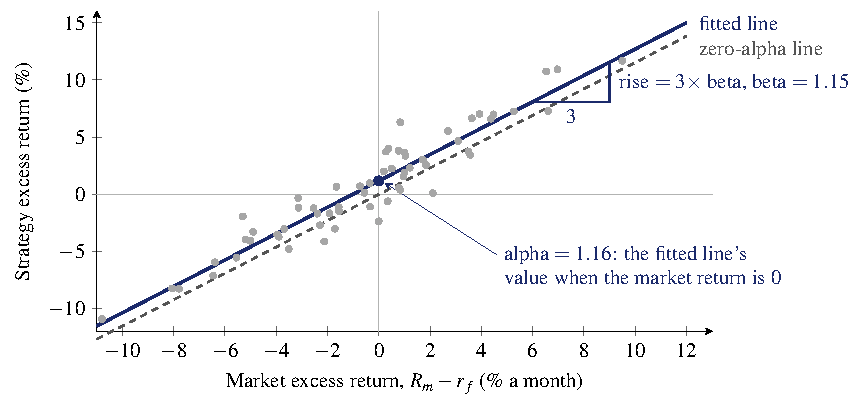
\includegraphics[width=0.85\linewidth]{images/fig03-1-regression-alpha.pdf}
%\caption{Beta and alpha in a regression of a strategy's monthly excess returns on the market's. Beta is the slope of the fitted line; alpha is its height where the market's excess return is zero, the gap between the fitted line and a line with the same slope through the origin. Simulated data, with an alpha larger than any real strategy's so that it is visible.}
%\label{fig:03-alpha}
%\end{figure}

\subsection{Multifactor models}
\label{sec:03-factors}

The CAPM fits the data poorly: small stocks and value stocks\index{value versus growth} have earned more than their betas imply (Chapter~\ref{ch:08}). \textbf{Factor models}\index{factor model|textbf} add further sources of risk, called factors. The Fama--French three-factor model adds two:

\begin{itemize}
  \item SMB\index{factor!SMB (size)} (small minus big): the return of small stocks over large ones;
  \item HML\index{factor!HML (value)} (high minus low): the return of value stocks, with high book-to-market ratios, over growth stocks, with low ones.
\end{itemize}

The model is
\begin{equation}
  R_i - r_f = \alpha_i + b_i(R_m - r_f) + s_i\,\mathrm{SMB} + h_i\,\mathrm{HML} + \varepsilon_i
  \label{eq:03-ff3}
\end{equation}
where $b_i$, $s_i$ and $h_i$ measure the asset's exposure to each factor. The factors are themselves \textbf{long--short} portfolio returns: each buys one group of stocks and sells the other short, so it costs roughly nothing to set up. A strategy's alpha relative to a factor model measures what it earns beyond its exposures to those factors.

\begin{callout}
\noindent \textbf{Contemporaneous decomposition of risk}

Notice that the factor model is a contemporaneous decomposition of risk. It asks how much asset $i$ moves together with the factors in the same period. 
The time-series factor regression is written with the same time index on both sides:
\begin{equation}
R_{i,t} - R_{f,t} = \alpha_i + \beta_i’ f_t + \varepsilon_{i,t}.
\end{equation}
The factors $f_t$ are themselves returns realized in period $t$, such as the market excess return, SMB, and HML. They are not known in advance, so they cannot be used to forecast anything. The regression is not trying to forecast. It measures exposure: $\beta_i$ is the covariance of asset $i$ with the factors, scaled by the factor variance. A high $R^2$ in this regression (often 90\% 
for diversified portfolios) says that the factors explain most of the asset’s variation.
\end{callout}

Two standard tools test whether a factor model works. The GRS test of Gibbons, Ross and Shanken (1989) asks whether the alphas of a whole set of portfolios are jointly zero. The \textbf{Fama--MacBeth}\index{regression!Fama--MacBeth|textbf} procedure (Fama and MacBeth 1973) asks a different question: do assets with more exposure to a factor earn higher average returns? Each month, it regresses the returns of many assets on their betas, and it then averages these monthly slopes over time. The average slope estimates the factor's reward, called its \textbf{risk premium}\index{risk premium|textbf}, and the variation of the slopes from month to month gives its standard error. Later chapters use both tools when they put specific factor models on trial.


\section{Stylized facts of financial returns}
\label{sec:03-facts}

The textbook standard error rests on three assumptions: observations are
independent, their variance is constant, and their distribution is roughly
normal. Real returns\index{real and nominal returns} depart from all three in consistent ways. This section
describes the four departures that matter most, and shows which assumption each
one breaks.

Decades of research have documented these features across markets, assets and
periods. Cont (2001) collected them as ``stylized facts,'' patterns found so
consistently that any model of returns must reproduce them:

\begin{enumerate}
  \item \textbf{Fat tails.}\index{fat tails|textbf} Extreme returns happen far more often than a normal distribution predicts (Figure~\ref{fig:03-tails}). Mandelbrot (1963) and Fama (1965) documented this in the 1960s. On October 19, 1987, the U.S. market fell by more than 20\% in a day, a move a normal distribution fitted to daily data would treat as essentially impossible. For daily stock index returns, kurtosis is typically far higher than the normal distribution's 3.
  \item \textbf{Volatility clustering.}\index{volatility clustering|textbf} Large moves tend to follow large moves, of either sign, and calm periods follow calm periods. Returns themselves show little autocorrelation, but their absolute values and squares are strongly and persistently autocorrelated. Chapter~\ref{ch:11} builds forecasting models on this feature.
  \item \textbf{Weak autocorrelation in returns.} Daily and monthly index returns show only small autocorrelations, consistent with Section~\ref{sec:01-efficient-markets}. Some portfolios, especially of small stocks, show more, partly because their prices are \textbf{stale}: some stocks do not trade every day, so their last recorded price lags the news.
  \item \textbf{Asymmetry.} Large falls are more common than large rises of the same size, and volatility tends to rise after falls. The rise in volatility after a fall is called the \textbf{leverage effect}\index{leverage effect|textbf}, because a falling share price raises a company's debt relative to its equity.
\end{enumerate}

%\begin{figure}[htbp]
%\centering
%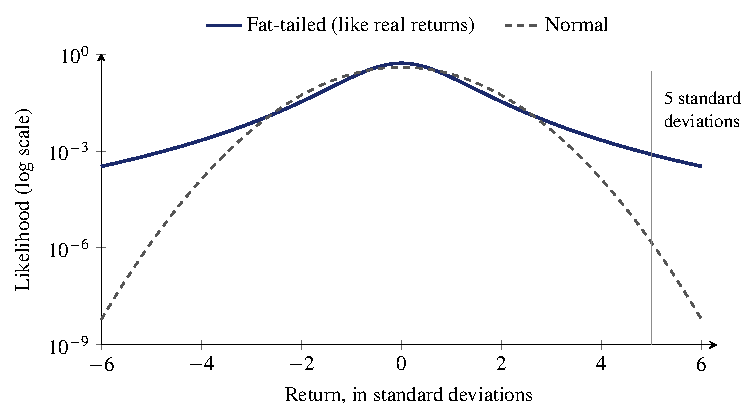
\includegraphics[width=0.85\linewidth]{images/fig03-2-fat-tails.pdf}
%\caption{Fat tails. Both curves have the same mean and standard deviation. On a log scale the difference in the tails becomes visible: a daily move of five standard deviations in either direction occurs about once in 7,000 years under the normal distribution, but about once every two years under the fat-tailed distribution shown, a Student-$t$ distribution with four degrees of freedom, which is a common model for daily returns.}
%\label{fig:03-tails}
%\end{figure}

\providecolor{fenavy}{HTML}{1B2A6B}
\providecolor{fegray}{HTML}{4D4D4D}

\begin{figure}[!htbp]
  \centering
  \begin{tikzpicture}[
    % Both densities have mean 0 and standard deviation 1.
    % Fat-tailed: Student t with 4 degrees of freedom, rescaled to unit
    % variance, whose density is sqrt(2) * (3/8) * (1 + x^2/2)^(-5/2).
    declare function={
      fat(\x)  = sqrt(2)*0.375*(1 + \x*\x/2)^(-2.5);
      norm(\x) = exp(-\x*\x/2)/sqrt(2*pi);
    }]
  % Panel (a): the whole distribution
  \begin{axis}[
    name=pa,
    scale only axis, width=0.29\linewidth, height=0.23\linewidth,
    axis lines=left, axis line style={-stealth, thin},
    xmin=-4.5, xmax=4.5, ymin=0, ymax=0.6,
    xtick={-4,-2,0,2,4}, ytick={0,0.2,0.4},
    yticklabel style={/pgf/number format/fixed},
    tick label style={font=\footnotesize}, label style={font=\small},
    xlabel={Return, in standard deviations}, ylabel={Density},
    title={(a) The whole distribution}, title style={font=\small},
    samples=200, domain=-4.5:4.5,
    legend style={draw=none, font=\footnotesize, at={(1.22,1.24)}, anchor=south,
                  legend columns=2, /tikz/every even column/.append style={column sep=1em}},
    clip=false,
  ]
    \addplot[fegray, thick, dashed] {norm(x)};
    \addlegendentry{Standard normal}
    \addplot[fenavy, very thick] {fat(x)};
    \addlegendentry{Fat-tailed (like real returns)}
    \node[fenavy, font=\footnotesize, anchor=west, align=left] at (axis cs:0.45,0.5)
      {taller,\\narrower peak};
    % Box marking the region enlarged in panel (b)
    \draw[gray!70, thin] (axis cs:3,-0.005) rectangle (axis cs:4.5,0.03);
  \end{axis}

  % Panel (b): close-up of the right tail
  \begin{axis}[
    at={(pa.east)}, anchor=west, xshift=1.7cm,
    scale only axis, width=0.29\linewidth, height=0.23\linewidth,
    axis lines=left, axis line style={-stealth, thin},
    xmin=3, xmax=6.2, ymin=0, ymax=0.008,
    xtick={3,4,5,6}, ytick={0,0.002,0.004,0.006,0.008},
    yticklabel style={/pgf/number format/fixed, /pgf/number format/precision=3},
    scaled y ticks=false,
    tick label style={font=\footnotesize}, label style={font=\small},
    xlabel={Return, in standard deviations},
    title={(b) Close-up of the right tail}, title style={font=\small},
    samples=150, domain=3:6.2,
    clip=false,
  ]
    \addplot[name path=fatc, fenavy, very thick] {fat(x)};
    \addplot[name path=normc, fegray, thick, dashed] {norm(x)};
    \path[name path=base] (axis cs:3,0) -- (axis cs:6.2,0);
    \addplot[fenavy!20] fill between[of=fatc and base, soft clip={domain=3:6.2}];
    \addplot[fenavy, very thick, domain=3:6.2] {fat(x)};

    \node[fenavy, font=\footnotesize, anchor=south west, align=left] at (axis cs:4.1,0.0042)
      {fat tail: extreme moves\\remain possible};
    \draw[fenavy, thin] (axis cs:4.15,0.0042) -- (axis cs:3.8,{fat(3.8)+0.0001});
  \end{axis}
  \end{tikzpicture}
  \caption{Fat tails. Both distributions have a mean of zero and a standard deviation of one. (a)~On an ordinary scale the two look similar, although the fat-tailed distribution has a taller, narrower peak. (b)~The difference lies in the tails. Beyond three standard deviations, the fat-tailed curve (shaded) stays well above the normal one, which falls almost to zero; at four standard deviations it is about 16 times higher. A daily move of five standard deviations in either direction occurs about once in 7,000 years under the normal distribution, but about once every two years under the fat-tailed distribution shown, a Student-$t$ distribution with four degrees of freedom, which is a common model for daily returns.}
  \label{fig:03-tails}
\end{figure}



The failure of the normal distribution has inspired a large body of research on methods that do not depend on it. One important family of tools is \textbf{Markov chain Monte Carlo}\index{Markov chain Monte Carlo|textbf} (MCMC), which simulates outcomes by drawing random samples step by step, with each draw depending on the one before it. MCMC lets researchers work with probability models that have no simple formula, such as returns with fat tails or volatility that changes over time (Jacquier, Polson and Rossi 1994). Kuo (2025, Chapter 14) introduces two MCMC algorithms, Gibbs sampling and the Metropolis--Hastings algorithm, and uses each of them to simulate 1,000 possible price paths for a stock over 200 trading days, starting from a price of \$100 (Figure~\ref{fig:03-mcmc-paths}). The two panels show how strongly the simulated future depends on the way returns are generated. In panel~(a), each day's return is drawn independently, and the paths spread out fairly evenly around the starting price. In panel~(b), each day's return depends on the previous day's, as it does in a Markov chain, and a few paths drift to more than ten times the starting price. Section~\ref{sec:03-bootstrap} introduces the bootstrap, a related method that simulates from the data themselves rather than from a model.

\begin{figure}[!htbp]
  \centering
  \begin{minipage}[t]{0.48\linewidth}
    \centering
    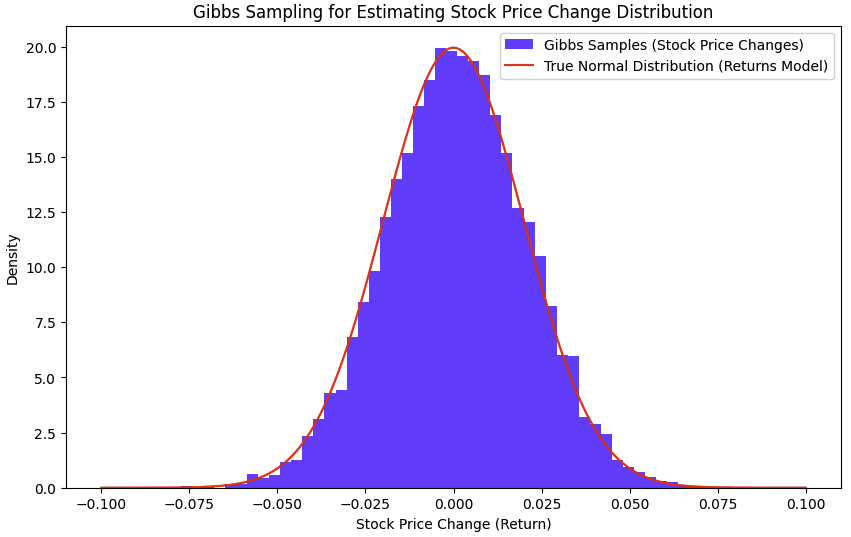
\includegraphics[width=\linewidth]{images/fig03-kuo-gibbs.png}\\[2pt]
    {\small (a) Gibbs sampling}
  \end{minipage}\hfill
  \begin{minipage}[t]{0.48\linewidth}
    \centering
    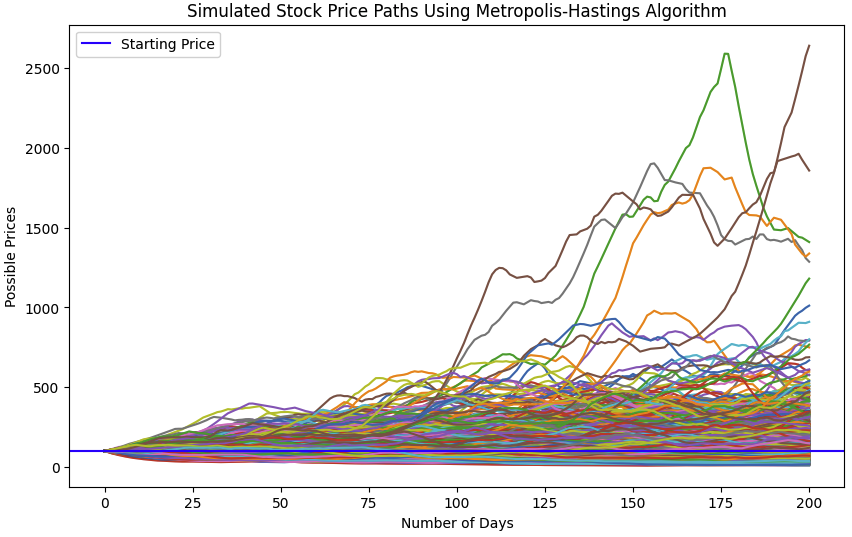
\includegraphics[width=\linewidth]{images/fig03-kuo-mh.png}\\[2pt]
    {\small (b) Metropolis--Hastings algorithm}
  \end{minipage}
  \caption{Simulated stock price paths from two MCMC algorithms, each showing 1,000 paths over 200 trading days from a starting price of \$100 (horizontal line). (a)~With Gibbs sampling, each day's return is drawn independently, and the paths spread evenly around the starting price. (b)~With the Metropolis--Hastings algorithm, each day's return depends on the previous day's, and a few paths rise far above the rest. Note the different vertical scales. Source: Kuo (2025), Figures 14.6 and 14.10.}
  \label{fig:03-mcmc-paths}
\end{figure}

\textbf{Why this matters for statistics.} None of these features biases the
regression estimates themselves, which usually remain right on average. What
they damage is the stated precision of those estimates, and with it every
t-statistic and \textbf{p-value}\index{p-value|textbf}, the probability of a result at least this
extreme if the true effect were zero. Each feature breaks a
different assumption, and the rest of the chapter deals with each in turn:

\begin{center}
\small
\begin{tabularx}{0.95\linewidth}{@{}>{\raggedright\arraybackslash}p{0.26\linewidth}>{\raggedright\arraybackslash}X>{\raggedright\arraybackslash}p{0.33\linewidth}@{}}
\toprule
Feature & Assumption it breaks & Remedy \\
\midrule
Volatility clustering & Constant variance & White or Newey--West standard errors (Section~\ref{sec:03-se}) \\
Autocorrelation and stale prices & Independence & Newey--West standard errors (Section~\ref{sec:03-se}) \\
Overlapping research designs & Independence, severely & Newey--West with enough lags, or Hodrick (1992) (Section~\ref{sec:03-overlap}) \\
Fat tails & Normality, so small-sample p-values are off & The bootstrap (Section~\ref{sec:03-bootstrap}) \\
\bottomrule
\end{tabularx}
\end{center}

\section{Choosing the right standard error}
\label{sec:03-se}

The estimates from a regression are usually reliable even when returns violate
the textbook assumptions. Their standard errors are not. The right standard
error is the one that allows for the dependence your data actually have: errors
whose variance changes over time, errors that move together over time, or
errors that move together across firms.

Consider the regression that appears throughout this book, a time-series
regression of a portfolio's excess return on one or more factors:
\begin{equation}
  r_t = \alpha + \beta' f_t + \varepsilon_t
  \label{eq:03-ts}
\end{equation}
where $f_t$ is the list of factor returns in month $t$ and $\beta'$ the list of
the portfolio's exposures to them. The classical standard error assumes that
the errors $\varepsilon_t$ are independent and equally variable. Three
alternatives relax these assumptions one step at a time:

\begin{itemize}
  \item \textbf{White (1980)}\index{standard error!robust (White)|textbf} allows the variance of the errors to change over
  time, as it does when volatility clusters.
  \item \textbf{Newey--West (1987)}\index{standard error!Newey--West (HAC)|textbf} also allows errors up to $L$ periods apart
  to be correlated. It is called a \textbf{HAC} estimator, for
  \emph{heteroskedasticity and autocorrelation consistent}.
  \item \textbf{Clustered} standard errors allow errors within a group, such as
  all firms in the same month, to be correlated (Petersen 2009).
\end{itemize}

\textbf{Which to use.} Match the standard error to the data:

\begin{center}
\small
\begin{tabularx}{0.95\linewidth}{@{}>{\raggedright\arraybackslash}p{0.34\linewidth}>{\raggedright\arraybackslash}p{0.28\linewidth}>{\raggedright\arraybackslash}X@{}}
\toprule
Your data & Use & Why \\
\midrule
Monthly returns, no overlap & White, or Newey--West with a few lags & Volatility changes, but errors are close to independent \\
Errors correlated over time (daily data, stale prices, persistent predictors) & Newey--West & Nearby errors move together \\
Overlapping $k$-period returns & Newey--West with at least $k-1$ lags, or Hodrick (1992) & The overlap builds in correlation $k-1$ periods long (Section~\ref{sec:03-overlap}) \\
Many firms over many periods & Clustered by firm and by time & Errors move together within a month and within a firm \\
\bottomrule
\end{tabularx}
\end{center}

When in doubt, report Newey--West. If the data have no dependence, it gives
almost the same answer as the classical formula, so little is lost; if they
do, it protects you from false confidence. Part B of the lab shows the first
case and Part C the second.

\textbf{Choosing the lag.} Newey--West needs one setting, the number of lags
$L$. A common rule of thumb is $L = \lfloor 4(T/100)^{2/9} \rfloor$, where
$\lfloor\cdot\rfloor$ means rounding down: 50 years of monthly data, $T = 600$,
gives $L = 5$. When the design creates dependence of a known length, such as
$k$-month overlapping returns, use at least $k - 1$ lags.

\textbf{How Newey--West works.} For readers who want the detail: every
standard error rests on an estimate of how much the regression's errors vary
and move together. Newey--West estimates it as
\begin{equation}
  \hat S = \sum_t x_t x_t' \hat\varepsilon_t^2 + \sum_{\ell=1}^{L} \left(1 - \frac{\ell}{L+1}\right) \sum_t \left(x_t \hat\varepsilon_t \hat\varepsilon_{t-\ell} x_{t-\ell}' + x_{t-\ell} \hat\varepsilon_{t-\ell} \hat\varepsilon_t x_t'\right)
  \label{eq:03-nw}
\end{equation}
where $x_t$ holds the regressors in period $t$. The first sum is White's
estimator, which lets each period have its own variance. The second adds the
correlations between errors up to $L$ periods apart, with weights that shrink
as the gap $\ell$ grows.

\section{Overlapping observations: less data than it seems}
\label{sec:03-overlap}

Long-horizon regressions became one of the most popular designs in return-prediction research. There are four good reasons for their appeal.

\begin{enumerate}
  \item \textbf{Valuation theory predicts returns over years, not months.} The dividend yield\index{valuation ratios!dividend yield} is dividends divided by price. When prices are high relative to dividends, one of two things must follow: dividends grow quickly, or future returns are low. Campbell and Shiller (1988) showed that this link is exact. Because dividends are hard to forecast, a high price today should be followed by low returns over the coming years, not necessarily in the next month.
  \item \textbf{Over long horizons, a small signal adds up faster than the noise.} Suppose a high dividend yield tells us that the market will earn 0.2\% a month more than usual. That extra return is the signal. The rest of the month's return is random noise, which moves the market up or down by about 4.5\% in a typical month. In a single month, the signal is therefore about one-twentieth the size of the noise, and it is almost impossible to see. Now add up 60 months. The signal is the same every month, so it simply adds up to $60 \times 0.2\% = 12\%$. The noise is random, so good and bad months partly cancel out, and it grows only to about $4.5\% \times \sqrt{60} \approx 35\%$. Over five years, the signal is about one-third the size of the noise, which makes it much easier to see. The signal therefore becomes easier to see at long horizons, and the $R^2$ rises from about 1\% at one month to 30\% or more at five years.
  \item \textbf{Long-term investors want forecasts for the next five or ten years.} Pension funds, endowments and people saving for retirement want to know whether the next five or ten years will be good or bad. A regression of five-year returns answers that question directly.
  \item \textbf{The design tests whether prices swing back after large moves.} In the late 1980s, Fama and French (1988) and Poterba and Summers (1988) asked whether stock prices tend to swing back after large moves. Long-horizon regressions were the natural tool for that test.
\end{enumerate}

The design also requires overlapping observations. Fifty years of data contain only ten separate five-year periods, which are too few for a regression, so researchers start a new five-year window every month and obtain about 600 observations. This uses all the data, but consecutive windows share 59 of their 60 months, so the 600 observations carry roughly the information of ten. Here lies the irony of the design. The feature that makes it attractive, a signal that adds up over time, is also what makes it misleading, because overlap and a persistent predictor make the $R^2$ and the t-statistic grow with the horizon even when there is no predictability at all. A real effect and a statistical artifact can look exactly the same, and the rest of this section explains how to tell them apart.

\textbf{The long-horizon regression.} A popular design in return-prediction research regresses
returns over a long horizon, such as the next five years, on a predictor
measured today, such as the dividend yield:
\begin{equation}
  r_{t+1} + r_{t+2} + \dots + r_{t+k} = a + b\,x_t + u_{t+k}
  \label{eq:03-longhorizon}
\end{equation}

\textbf{Overlapping returns hold far fewer independent observations than they appear to.} With monthly data and $k = 60$,
each observation's dependent variable shares 59 of its 60 months with the next
observation's (Figure~\ref{fig:03-overlap}). The regression appears to have
hundreds of observations but contains roughly $T/k$ independent ones. Fifty
years of monthly data, $T = 600$, give only $600/60 = 10$ independent five-year
returns.

%\begin{figure}[htbp]
%\centering
%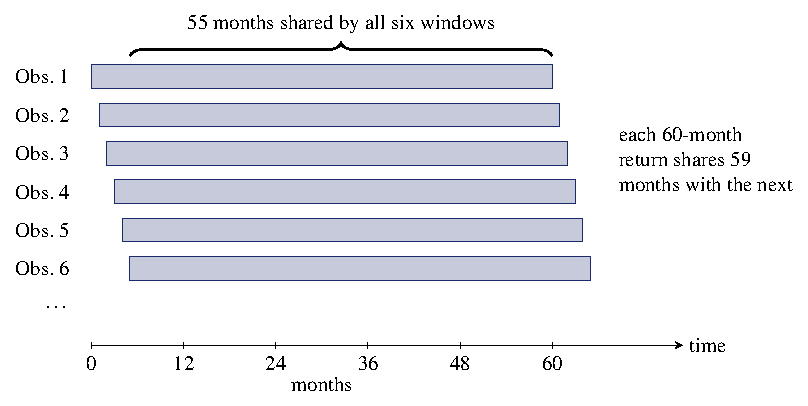
\includegraphics[width=0.85\linewidth]{images/fig03-3-overlap.pdf}
%\caption{Overlapping observations. Each observation in a regression of five-year returns covers 60 months, and each starts one month after the last. Consecutive observations share 59 of their 60 months, so they carry almost the same information.}
%\label{fig:03-overlap}
%\end{figure}


\providecolor{fenavy}{HTML}{1B2A6B}

\begin{figure}[!htbp]
  \centering
  \begin{tikzpicture}[x=0.115cm, y=0.62cm]
    % Six overlapping 60-month windows; window i covers months i-1 to i+59
    \foreach \wfI in {1,...,6} {
      \pgfmathsetmacro{\wfS}{\wfI-1}
      \filldraw[fill=fenavy!25, draw=fenavy!70]
        (\wfS,-\wfI+0.32) rectangle (\wfS+60,-\wfI-0.32);
      \node[anchor=east] at (-2,-\wfI) {Obs.~\wfI};
    }
    \node[anchor=east] at (-2,-7) {\dots};

    % Months shared by all six windows: 5 to 60
    \draw[decorate, decoration={brace, amplitude=5pt}] (5,-0.45) -- (60,-0.45)
      node[midway, above=6pt] {55 months shared by all six windows};

    % Note on the right
    \node[anchor=west, align=left] at (68,-3.2)
      {each 60-month\\return shares 59\\months with the next};

    % Time axis
    \draw[-stealth, thin] (0,-8.2) -- (79,-8.2) node[anchor=west] {time};
    \foreach \wfT in {0,12,24,36,48,60} {
      \draw (\wfT,-8.1) -- (\wfT,-8.3);
      \node[anchor=north] at (\wfT,-8.3) {\wfT};
    }
    \node at (30,-9.5) {months};
  \end{tikzpicture}
\caption{Overlapping observations. Each observation in a regression of five-year returns covers 60 months, and each starts one month after the last. Consecutive observations share 59 of their 60 months, so they carry almost the same information.}
\label{fig:03-overlap}
\end{figure}



\textbf{Overlap and persistence\index{persistence} cause two problems.}

\begin{enumerate}
  \item \textbf{Overlap makes classical standard errors far too small.} The errors $u$ are strongly autocorrelated by construction, up to lag $k - 1$. Classical standard errors ignore this and can be several times too small. Hansen and Hodrick (1980) and Newey--West correct for the overlap, but in samples of typical length they still reject a true null hypothesis\index{hypothesis testing!null hypothesis} too often. A test's \textbf{size} is the rate at which it does so; a well-behaved 5\% test has a size of 5\%. Hodrick (1992) proposed an alternative that avoids overlapping errors and has more reliable size.
  \item \textbf{Persistent predictors bias the estimated slope.} A variable is \textbf{persistent} when it moves slowly, so that this month's value is close to last month's. The dividend yield has a monthly autocorrelation close to 1. Stambaugh\index{Stambaugh bias} (1999) showed that when the predictor's surprises are correlated with return surprises, as they are for valuation ratios, the estimated slope is biased in finite samples. Valkanov (2003) showed that with overlapping horizons and persistent predictors, t-statistics do not even converge to the normal distribution, so the usual critical values are wrong.
\end{enumerate}

\textbf{A rising $R^2$ at longer horizons is not evidence of predictability.} $R^2$ tends to rise with the horizon
even when there is no predictability at all. Long-horizon regressions
mechanically add up the same short-horizon information, so a rising $R^2$ does
not by itself show that returns become more predictable in the long run.

\textbf{How to read a long-horizon result.} Before you trust one, take these four steps:

\begin{itemize}
  \item count the independent observations, roughly $T/k$, before reading any t-statistic;
  \item use Newey--West with at least $k-1$ lags, or better, Hodrick's (1992) method;
  \item check the one-period regression first: a long-horizon result adds little if the one-period evidence is weak;
  \item treat persistent predictors, such as valuation ratios, with extra caution.
\end{itemize}

\begin{callout}
\textbf{What Failed: the long-horizon evidence.} In the late 1980s and 1990s, regressions of multi-year returns on dividend yields reported $R^2$ values of 30\% or more and large t-statistics, and were widely read as strong evidence that stock returns are predictable\index{return predictability} over long horizons. Later work showed how much of that strength came from the design. Valkanov (2003) and Boudoukh, Richardson and Whitelaw (2008) argued that, once overlap and persistence are accounted for, long-horizon regressions add little beyond what the one-period regression already shows, and that one-period evidence is weak. Chapter~\ref{ch:07} tests return predictability directly; the lab in this chapter shows the statistical mechanism.
\end{callout}

\section{The bootstrap: uncertainty without a formula}
\label{sec:03-bootstrap}

Every standard error so far in this chapter comes from a formula, and every formula rests on assumptions about how returns behave. Section~\ref{sec:03-facts} described one way around such formulas, Markov chain Monte Carlo, which simulates many possible outcomes from a probability model chosen by the researcher. Its results, however, can be no better than that model. The \textbf{bootstrap}\index{bootstrap|textbf}, introduced by Efron (1979), takes a different route. Instead of simulating from a model, it resamples the data themselves and recomputes the statistic of interest on each resampled version. Because the resampled data come from the real returns, fat tails and other features of those returns are carried into the answer automatically, and no formula is needed.

\textbf{The recipe.} The basic bootstrap takes four steps.

\begin{enumerate}
  \item Draw $T$ observations at random from the sample \textbf{with replacement}, so that some observations appear more than once and others not at all.
  \item Recompute the statistic, such as a Sharpe ratio\index{Sharpe ratio} or an alpha, on this new sample.
  \item Repeat these two steps a few thousand times.
  \item Use the spread of the recomputed values as the standard error, or read a confidence interval\index{confidence interval} from their percentiles.
\end{enumerate}

\textbf{For returns, resample blocks rather than single months.} If individual months are drawn at random, any dependence over time is destroyed, including volatility clustering, and the bootstrap understates the uncertainty. For time series, the bootstrap therefore resamples blocks of consecutive observations. There are two common versions.

\begin{itemize}
  \item The \textbf{moving-block bootstrap}\index{bootstrap!moving-block|textbf} draws blocks of a fixed length $b$.
  \item The \textbf{stationary bootstrap}\index{bootstrap!stationary|textbf} of Politis and Romano (1994) draws blocks of random length, with an average length of $b$. This keeps the resampled series \textbf{stationary}\index{stationarity|textbf}, which means that its statistical properties do not depend on the date. It is the default in this book.
\end{itemize}

When a regression involves several series, such as a portfolio and the factors, the bootstrap must resample entire rows together, so that the relationships between the series are preserved.

\textbf{The bootstrap is most useful when no reliable formula exists.} Typical uses include confidence intervals for Sharpe ratios and alphas when returns have fat tails, and tests of whether the best performers in a group did better than luck alone would produce. Kosowski, Timmermann, Wermers and White (2006) and Fama and French (2010) used it in this way to ask whether the top mutual fund managers have genuine skill, which is an empirical version of the random strategies in Lab~\ref{ch:01}.

\textbf{The bootstrap cannot create information that the sample lacks.} Because it only reshuffles the observed data, it can reflect only what the sample contains. If the sample is short, or if it contains a single rare event such as one crash, the resampled data will show that event only as often as it appeared in the sample, and no more.

\section{The best of many strategies: White's reality check}
\label{sec:03-reality}

Lab~\ref{ch:01} showed that the best of many strategies can look impressive by luck alone, and Chapter~\ref{ch:01} dealt with the problem by raising the hurdle for the t-statistic as the number of strategies grows. White (2000) proposed a more direct test that builds on the bootstrap. His \textbf{reality check}\index{White's reality check|textbf} asks whether the best of many strategies truly beats a benchmark, such as buying and holding the market, once the search that found it is taken into account. The test takes four steps.

\begin{enumerate}
  \item Measure each strategy's average performance relative to the benchmark, and record the best of these values.
  \item Resample the data with the stationary bootstrap, drawing the same blocks of months for every strategy at once, so that the correlations between the strategies are preserved.
  \item In each resampled history, shift every strategy's performance so that none of them has any true advantage over the benchmark, and record the best performance among them. Repeated a few thousand times, this shows how good the best strategy would look by luck alone.
  \item Compare the actual best performance with these luck-only results. If it beats, for example, 95\% of them, the winner outperforms the benchmark even after allowing for the search.
\end{enumerate}

Two features make the reality check valuable. It uses every strategy that was tried, so the size of the search is built into the test. It also resamples all the strategies together, so near-copies of the same rule count for less than truly different ones, without any need to count how many independent bets they contain. Hansen (2005) refined the test into the \textbf{test of superior predictive ability\index{test of superior predictive ability}} (SPA), which is less easily weakened when many poor or irrelevant strategies are included in the comparison. Both tests share one requirement: they need the returns of every strategy that was tried, including those that were abandoned. A researcher who has not kept a record of every trial cannot run them.

\begin{callout}
\textbf{What Failed: a century of technical trading rules.} Brock, Lakonishok and LeBaron (1992) found that simple moving-average and trading-range rules applied to the Dow Jones index from 1897 to 1986 produced significant profits. Sullivan, Timmermann and White (1999) re-examined them against a universe of several thousand related rules, using White's reality check to account for the search. The best rule still looked significant in the original sample, but its superior performance did not carry over to the decade that followed. A result that survives a search can still fail the test that matters most, which is new data.
\end{callout}

\section{Statistical versus economic significance}
\label{sec:03-economic}

A result can be statistically significant and still not worth acting on, and a
result worth acting on can fail to be significant. Before believing or
dismissing any finding, ask two separate questions: is it real, and is it
large enough to matter?

A t-statistic answers only the first: how surprising would this estimate be if
the true effect were zero? An effect is \textbf{statistically significant}\index{statistical significance|textbf} if it
is unlikely to be due to chance, and \textbf{economically significant}\index{economic significance|textbf} if it is
large enough to change what an investor would do. The two can diverge in both
directions:

\begin{center}
\small
\begin{tabularx}{0.9\linewidth}{@{}>{\raggedright\arraybackslash}p{0.20\linewidth}>{\raggedright\arraybackslash}X>{\raggedright\arraybackslash}X@{}}
\toprule
 & Economically small & Economically large \\
\midrule
\textbf{Statistically significant} & A tiny alpha measured precisely, such as 0.5\% a year on a low-risk, high-turnover strategy whose costs exceed it & The claims worth acting on, if they survive the rest of the book's tests \\
\textbf{Not significant} & Nothing to see & A large alpha measured imprecisely, such as 6\% a year over a short, volatile record (Section~\ref{sec:01-signal-noise}) \\
\bottomrule
\end{tabularx}
\end{center}

Three habits keep the two apart:

\begin{enumerate}
  \item \textbf{Always report the size of the effect in units that matter}: percent per year, dollars, or a change in Sharpe ratio, alongside the t-statistic.
  \item \textbf{Compare the effect with what it costs to capture.} A return spread that requires monthly rebalancing\index{rebalancing} of illiquid stocks may vanish after costs (Chapter~\ref{ch:06}).
  \item \textbf{Read a confidence interval, not just a p-value.} A 95\% \textbf{confidence interval}\index{confidence interval|textbf} is a range that, in repeated samples, would contain the true value 95\% of the time. An interval of ``1\% to 11\% a year'' says more than ``$p = 0.02$'': the effect could be negligible or enormous.
\end{enumerate}

Harvey (2017), in his presidential address to the American Finance Association, argued that the field's emphasis on crossing $p < 0.05$ encourages exactly the behaviors that Chapter~\ref{ch:01} describes, and that researchers should combine statistical evidence with prior plausibility and economic magnitude. This book's verdicts follow that advice: no claim survives on a t-statistic alone.

\section{Lab~\thechapter: When a t-statistic's assumptions fail}
\label{sec:03-lab}

\begin{callout}
\textbf{Lab~\ref{ch:03} at a glance.} \emph{Claim on trial:} with the right standard errors, regression statistics are reliable for financial returns. \emph{Data:} daily and monthly U.S. market returns and the 25 Fama--French portfolios formed on size and book-to-market, from the Kenneth R. French Data Library\index{Kenneth French data library} (downloaded automatically). \emph{Tools:} Python with pandas, NumPy, SciPy and matplotlib, plus the fintest module. \emph{Time:} about two hours, including the guided notebook. \emph{Code:} repository folder \texttt{ch03-noisy-returns/}.
\end{callout}

The design of this lab draws on several well-known studies, each of which showed how the features of returns affect statistical evidence. Part~A measures the stylized facts that Mandelbrot (1963) and Fama (1965) first documented and that Cont (2001) later summarized. Part~B uses the 25 portfolios of Fama and French (1993), the standard test assets in empirical asset pricing, and compares the classical standard error with the corrections of White (1980), Newey and West (1987) and the stationary bootstrap of Politis and Romano (1994). Part~C follows the simulation experiments of Hodrick (1992) and Valkanov (2003), who showed that overlapping long-horizon regressions find predictability far too often when none exists, and it lets readers add the bias that Stambaugh (1999) identified for persistent predictors. Part~D takes up the point that Harvey (2017) made in his presidential address to the American Finance Association, that statistical significance alone is not enough. Each part repeats the logic of these studies with free data, so that you can see each problem for yourself.


\subsection*{Part A: Stylized facts}

The lab measures the skewness and kurtosis of daily and monthly market returns, counts the days beyond 3, 4, 5 and 6 standard deviations against what a normal distribution would predict, and plots the autocorrelations of returns and of absolute returns over 50 trading days (Lab Figures~\ref{ch:03}.1 and~\ref{ch:03}.2). Readers should expect returns themselves to show little memory and their absolute size to show a great deal: volatility clustering in one picture.

\subsection*{Part B: Four standard errors for 25 alphas}

The 25 portfolios formed on size and book-to-market are the classic \textbf{test assets}\index{factor!test assets|textbf} of Fama and French (1993): the portfolios whose returns a model must explain. From July 1963 onward, the lab estimates each portfolio's alpha under the CAPM and the three-factor model and computes four t-statistics: classical, White, Newey--West and stationary bootstrap. It reports how many alphas are significant under each method and the typical ratio of robust to classical standard errors (Lab Figure~\ref{ch:03}.3).

This part is designed to show where corrections matter \textbf{less}. Monthly portfolio returns have little autocorrelation and no overlap, so the four methods should usually agree closely. That is itself a finding: robust standard errors are cheap insurance, not a guarantee of different answers.

\subsection*{Part C: Overlapping regressions with a useless predictor}

This part is a controlled experiment. It takes the real monthly market returns and pairs them with 1,000 simulated predictors that behave like a dividend yield (monthly autocorrelation 0.98) but have \textbf{no} predictive power, by construction. For horizons from 1 to 60 months, it runs the long-horizon regression of Equation~\eqref{eq:03-longhorizon} for every predictor and records how often each method finds a ``significant'' slope (Lab Figure~\ref{ch:03}.4).

Because the truth is known, a correct test should reject about 5\% of the time at every horizon. Theory and the earlier literature lead readers to expect classical t-statistics to reject far more often as the horizon grows, Newey--West to do better but still reject too often at long horizons, and Hodrick's (1992) method to stay close to 5\%. The same figure shows the average $R^2$ of these useless predictors rising with the horizon.

An option sets the correlation between the predictor's surprises and return surprises, so readers can add the Stambaugh (1999) bias to the experiment and watch the slope estimates shift.

\subsection*{Part D: Economic significance}

Finally, the lab plots each portfolio's three-factor alpha in percent per year with its 95\% bootstrap interval (Lab Figure~\ref{ch:03}.5), and counts alphas that are statistically significant but economically small, and alphas that are large but statistically indistinguishable from zero.

\emph{[Draft note: the figures and numbers for Parts A, B and D, and the real-return inputs to Part C, are generated from the Kenneth R. French data at the time of publication. The book prints those results; the text above describes only what theory predicts.]}

\subsection*{Your verdict}

Readers judge the claim by comparing the results of Parts B and C. The expected verdict is \textbf{survives, with conditions}, because the answer depends on the design of the regression.

\begin{enumerate}
  \item \textbf{When monthly returns do not overlap, the claim holds comfortably.} In Part B, the classical, White, Newey--West and bootstrap standard errors usually agree closely, so the choice among them makes little difference.
  \item \textbf{When the design builds in dependence, the claim holds only if the right standard error is chosen.} In Part C, classical t-statistics find far too many ``significant'' slopes. Newey--West standard errors help, but they still find too many at long horizons, while Hodrick's (1992) method keeps the error rate close to 5\%.
\end{enumerate}

The lesson is a rule that you can apply to any regression. First, match the standard error to the design of the study, using the table in Section~\ref{sec:03-se}. Second, report the size of the effect alongside its t-statistic. If you follow both steps, you can trust what a regression's statistics tell you.



\section{What investors can use}
\label{sec:03-investors}

Most investors will never compute a Newey--West standard error. But the ideas in this chapter translate directly into questions about any statistical claim.

\textbf{Rules of thumb}

\begin{enumerate}
  \item Ask how many independent observations stand behind a result. Fifty years of five-year returns is ten independent observations, not six hundred.
  \item Be wary of long-horizon claims with high $R^2$. Overlap and persistent predictors produce impressive $R^2$ values even when there is nothing to find.
  \item Translate every statistical result into money. A significant alpha smaller than the fund's fee is worth nothing to the investor.
  \item Remember that one t-statistic among many is not a discovery: across 25 portfolios, one or two will look significant by chance.
\end{enumerate}

\textbf{Questions to ask a fund manager or research provider}

\begin{itemize}
  \item What standard errors did you use, and do your results hold with ones robust to heteroskedasticity and autocorrelation?
  \item If you forecast over long horizons, how many non-overlapping periods does your sample contain?
  \item What is the confidence interval for the alpha or Sharpe ratio, not just its point estimate?
  \item How large is the effect after fees and trading costs\index{transaction costs}?
\end{itemize}

\section*{Exercises}
\addcontentsline{toc}{section}{Exercises}

\subsection*{Conceptual (all readers)}

\begin{enumerate}
  \item Daily market returns show almost no autocorrelation, yet their absolute values are strongly autocorrelated. Explain how both can be true, and why it matters for standard errors.
  \item A regression of five-year returns on the dividend yield uses 60 years of monthly data. Roughly how many independent observations does it contain? What would you expect of its classical t-statistic?
  \item Why must a bootstrap for time series resample blocks rather than individual months?
  \item A strategy has an alpha of 0.4\% a year with $t = 4.5$. Another has an alpha of 5\% a year with $t = 1.2$. Which would you investigate further, and what would you need to know?
\end{enumerate}

\subsection*{Lab extensions (technical readers)}

\begin{enumerate}
  \setcounter{enumi}{4}
  \item Part C: set the correlation between predictor surprises and return surprises to $-0.9$. What happens to the average estimated slope and to the rejection rates? Relate your answer to Stambaugh (1999).
  \item Part C: vary the predictor's autocorrelation (0.9, 0.98, 0.995). How does persistence affect false discoveries?
  \item Part B: use the full sample from 1926 and a Newey--West lag of 12. Which conclusions change?
  \item Apply White's (2000) reality check, with the stationary bootstrap, to the 1,000 random strategies of Lab~\ref{ch:01}. Does the test correctly find that the best of them has no skill? Then add one strategy with genuine skill, as in Lab extension 9 of Chapter~\ref{ch:01}, and see whether the test detects it.
\end{enumerate}
